\section{Origin}
Because this project is about shaping the directional characteristics of loudspeakers arrangements towards a particular direction, it is important to thorougly investigate the directional characteristic of a single loudspeaker cabinet. This serves as a baseline for comparison and also is essential, because the investigated cabinet will be used to form the speaker array later on.\\
In general, loudspeakers tend to display different directional behaviour depending on the frequency emitted. At low frequencies they can be viewed as omnidirectional sound sources. At higher frequencies the main direction of sound emission is in line with the motion direction of the voice coil. \citep[p. 910 f.]{crocker98}
Depending on the ratio of the emitted wavelength to the diameter of the speaker, a radiation pattern with side lobes can occur. An analytic approximation to the behaviour can be made  when looking at a vibrating piston in an infinite baffel. However, this only takes into account the front side of the speaker. It is difficult to incorporate the effects of an enclosure into this model.\\
There are possibilities to numerically model the sound field around a speaker in a cabinet. However in the context of this project, conducting a measurement seems to be the most favourable approach towards quantifying the sound pressure emitted by loudspeaker mounted in an enclosure. Measurements must be taken at numerous frequencies and positions along a circular trajectory.
For this project, measurements are conducted by placing the test object on a turntable in free field conditions and measuring transfer functions with a microphone. The voltage output of the amplifier and the gain of the microphone can be calibrated so that the only part unknown is transduction performed by the test object.
The knowledge gained through these measurements can then be used in order to designate a feasible frequency range for beamforming in the way that will be described later on. 

\section{Transfer Function Measurement with Sweeps}
The characterization of the directional behaviour of the speaker consists of a large number of transfer function measurements. While there are many methods available to obtain transfer functions, it was decided to go with a method that is based on sweeps, due to several benefits. \citep[p. 3 ff.]{mueller01}\\
The sweep signal used for the measurement can be generated by the \gls{ift} of a desired spectrum and a group delay that is designed accordingly. This results in a sinusidal waveform with a continuously altering frequency. In most cases it is desirable to keep a nearly constant amplitude over the whole length of the sweep. The procedure of generating such a sweep signal is illustrated in \autoref{fig:sweep_signal}.

\begin{figure}[htbp]
	\centering
	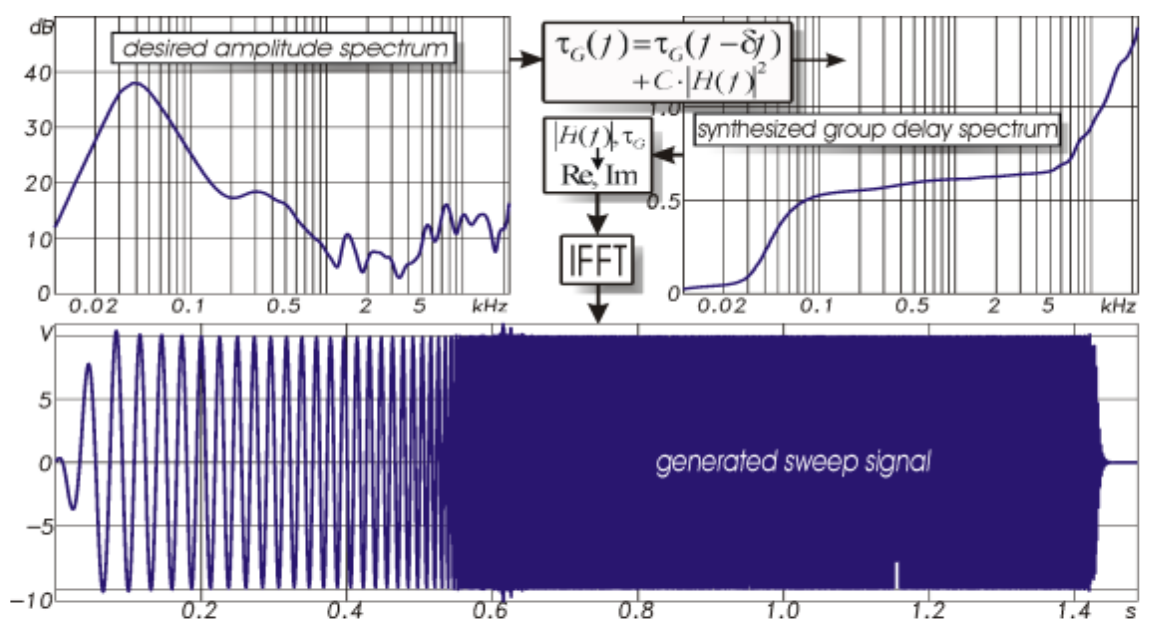
\includegraphics[width=1\textwidth]{mueller01_sweep.png}
	\caption{Sweep synthesis with arbitrary spectral magnitude and nearly constant envelope, taken from \citep{mueller01}}
		\label{fig:sweep_signal}
\end{figure}


The sweep signal is played back via the 